\section{Date: 2026-10-01}
\noindent \textbf{Series ID: W568RC1A027NBEA} 

\noindent This series is titled Government current receipts: Imputations and has a frequency of Annual. The units are Billions of Dollars and the seasonal adjustment is Not Seasonally Adjusted.The observation start date is 1929-01-01 and the observation end date is 2022-01-01.The popularity of this series is 1. \\ 

\noindent \textbf{Series ID: BOPOON} 

\noindent This series is titled U.S. Official Reserve Assets Abroad, Net (DISCONTINUED) and has a frequency of Quarterly. The units are Billions of Dollars and the seasonal adjustment is Not Seasonally Adjusted.The observation start date is 1960-01-01 and the observation end date is 2014-01-01.The popularity of this series is 1. \\ 

\subsection{Raw Regression}
\noindent Regresses the two series against each other directly. A significant result here can come just as easily from both series sharing a long-run trend as from any real relationship.

\begin{center}
\begin{tabular}{lclc}
\toprule
\textbf{Dep. Variable:}               & value\_fred\_BOPOON & \textbf{  R-squared:         } &     0.001   \\
\textbf{Model:}                       &         OLS         & \textbf{  Adj. R-squared:    } &    -0.018   \\
\textbf{Method:}                      &    Least Squares    & \textbf{  F-statistic:       } &   0.04727   \\
\textbf{Date:}                        &   Thu, 01 Oct 2026  & \textbf{  Prob (F-statistic):} &    0.829    \\
\textbf{Time:}                        &       19:55:13      & \textbf{  Log-Likelihood:    } &   -112.57   \\
\textbf{No. Observations:}            &            55       & \textbf{  AIC:               } &     229.1   \\
\textbf{Df Residuals:}                &            53       & \textbf{  BIC:               } &     233.1   \\
\textbf{Df Model:}                    &             1       & \textbf{                     } &             \\
\textbf{Covariance Type:}             &      nonrobust      & \textbf{                     } &             \\
\bottomrule
\end{tabular}
\begin{tabular}{lcccccc}
                                      & \textbf{coef} & \textbf{std err} & \textbf{t} & \textbf{P$> |$t$|$} & \textbf{[0.025} & \textbf{0.975]}  \\
\midrule
\textbf{const}                        &      -0.2012  &        0.458     &    -0.439  &         0.662        &       -1.119    &        0.717     \\
\textbf{value\_fred\_W568RC1A027NBEA} &      -0.0115  &        0.053     &    -0.217  &         0.829        &       -0.117    &        0.094     \\
\bottomrule
\end{tabular}
\begin{tabular}{lclc}
\textbf{Omnibus:}       &  6.566 & \textbf{  Durbin-Watson:     } &    1.473  \\
\textbf{Prob(Omnibus):} &  0.038 & \textbf{  Jarque-Bera (JB):  } &   10.848  \\
\textbf{Skew:}          &  0.067 & \textbf{  Prob(JB):          } &  0.00441  \\
\textbf{Kurtosis:}      &  5.172 & \textbf{  Cond. No.          } &     15.6  \\
\bottomrule
\end{tabular}
%\caption{OLS Regression Results}
\end{center}

Notes: \newline
 [1] Standard Errors assume that the covariance matrix of the errors is correctly specified.

\begin{figure}
\centering
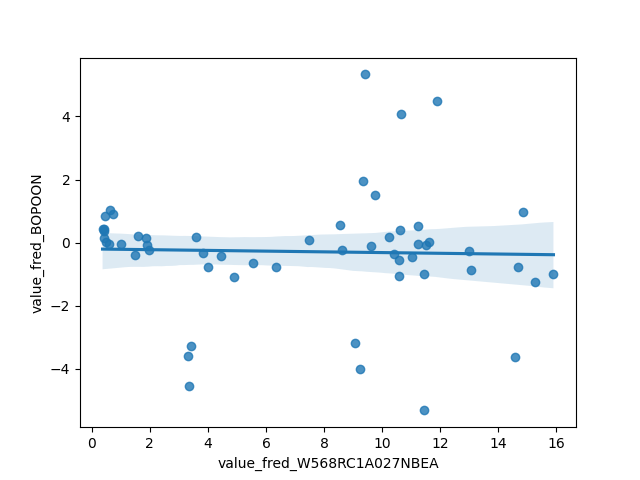
\includegraphics[scale = 0.9]{plots/plot_2026-10-01.png}
\caption{Raw Regression Plot for 2026-10-01}
\end{figure}
\newpage
\subsection{Detrended Regression}
\noindent Regresses the residuals of each series after removing its own linear time trend, so a shared trend can no longer drive the result on its own. A relationship that stays significant here is better evidence of a genuine link between the two series.

\begin{center}
\begin{tabular}{lclc}
\toprule
\textbf{Dep. Variable:}                          & value\_fred\_BOPOON\_detrended & \textbf{  R-squared:         } &     0.007   \\
\textbf{Model:}                                  &              OLS               & \textbf{  Adj. R-squared:    } &    -0.011   \\
\textbf{Method:}                                 &         Least Squares          & \textbf{  F-statistic:       } &    0.3913   \\
\textbf{Date:}                                   &        Thu, 01 Oct 2026        & \textbf{  Prob (F-statistic):} &    0.534    \\
\textbf{Time:}                                   &            19:55:13            & \textbf{  Log-Likelihood:    } &   -112.39   \\
\textbf{No. Observations:}                       &                 55             & \textbf{  AIC:               } &     228.8   \\
\textbf{Df Residuals:}                           &                 53             & \textbf{  BIC:               } &     232.8   \\
\textbf{Df Model:}                               &                  1             & \textbf{                     } &             \\
\textbf{Covariance Type:}                        &           nonrobust            & \textbf{                     } &             \\
\bottomrule
\end{tabular}
\begin{tabular}{lcccccc}
                                                 & \textbf{coef} & \textbf{std err} & \textbf{t} & \textbf{P$> |$t$|$} & \textbf{[0.025} & \textbf{0.975]}  \\
\midrule
\textbf{const}                                   &   -1.084e-14  &        0.256     & -4.22e-14  &         1.000        &       -0.514    &        0.514     \\
\textbf{value\_fred\_W568RC1A027NBEA\_detrended} &      -0.1030  &        0.165     &    -0.626  &         0.534        &       -0.433    &        0.227     \\
\bottomrule
\end{tabular}
\begin{tabular}{lclc}
\textbf{Omnibus:}       &  5.994 & \textbf{  Durbin-Watson:     } &    1.499  \\
\textbf{Prob(Omnibus):} &  0.050 & \textbf{  Jarque-Bera (JB):  } &    9.174  \\
\textbf{Skew:}          &  0.019 & \textbf{  Prob(JB):          } &   0.0102  \\
\textbf{Kurtosis:}      &  5.000 & \textbf{  Cond. No.          } &     1.56  \\
\bottomrule
\end{tabular}
%\caption{OLS Regression Results}
\end{center}

Notes: \newline
 [1] Standard Errors assume that the covariance matrix of the errors is correctly specified.

\begin{figure}
\centering
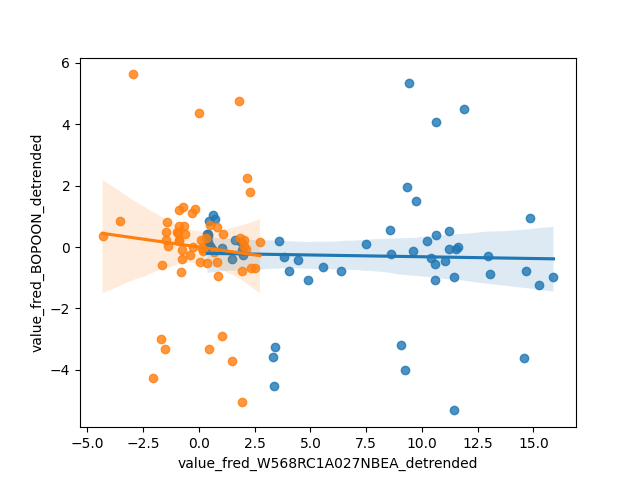
\includegraphics[scale = 0.9]{plots/plot_2026-10-01_detrended.png}
\caption{Detrended Regression Plot for 2026-10-01}
\end{figure}
\newpage
